\scanpage{155}
Si $C$ est plat sur $k$, et $s\hookrightarrow k^I$ pour $I$ convenable
i.e. $s\mathbin{\text{---}}k^{s^k}$ $(x\longmapsto(u(x))_{u\in s^k})$ est injectif,
alors $C\otimes s\mathbin{\text{---}}C\otimes_{\unsure{s|k}}k^I$ est injectif, mais
\diagram{\[
\begin{array}{rclll}
C\otimes_k k^{(I)}&\longrightarrow&(C\otimes_k k)^I=&C^I&\text{est-il injectif ?}\\
&&&\text{\textquotedbl}&\\
&&&\operatorname{Hom}(k^{(I)},C).&
\end{array}
\]}
\uline{Oui}, par passage à la limite inductive sur $I$, on se ramène au cas $I$ fini\unsure{---}.
\figure{
\begin{tikzpicture}\draw (0,0)--(.2,.5);\draw (.08,0)--(.28,.5);\end{tikzpicture}}
\unsure{Même conclusion} sans hyp. de platitude sur $C$ en supposant que $s$ est \uline{libre} sur $k$\ldots
\figure{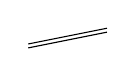
\begin{tikzpicture}\draw (0,0)--(1,.2);\draw (0,-.05)--(1,.15);\end{tikzpicture}}
\[
 s=k[U].\qquad s^k=k\{\{T\}\}
\]
structure de $k$-Alg. ordinaire
\[
 \begin{aligned}
 C&=k[U][Y_0,\ldots,Y_n]\\
  &=k[U,Y_0,\ldots,Y_n]
 \end{aligned}
 \qquad C^k=k\{\{T\}\}\{\{X_0,\ldots,X_n\}\}
\]
structure de $k$-Alg. ordinaire qui est une $s^k$-Alg.

$C^k$ opère sur $C$ par les
\[
 T^{(i)}X_0^{(i_0)}\cdots X_n^{(i_n)}
\]
qui \unsure{op. par} les op. diff.
\[
 D_U^{(i)}D_{Y_0}^{(i_0)}\cdots D_{Y_n}^{(i_n)}
\]
\deleted{\unsure{NB}} Donc $s^k$ opère par les $D_U^{(i)}$.

\uline{Remarque} Toutes ces opérations sont \inserted{loc.}\uline{nilpotentes}, de façon précise si $P\in C$ fixé, $P$ de degré $n$,
alors $D_fP=0$ si $f\in C^k$ est d'\uline{ordre} $>n$,
a fortiori si $f\in s^k$ d'ordre $>n$.
\figure{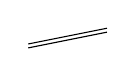
\begin{tikzpicture}\draw (0,0)--(1,.2);\draw (0,-.05)--(1,.15);\end{tikzpicture}}
Supposons $s$ $k$-coalgèbre (coassociatif, unitaire)
libre comme $k$-module, quelles sont les structures de $s^k$-algèbre sur \inserted{le $k$-module} $C$ qui
proviennent d'une structure de $k$-comodule ?
\diagram{\begin{tikzcd}[column sep=large]
 C\arrow[r] & C\otimes_k s\arrow[r,phantom,"\subset" description,"{\text{inj. car }s\text{ libre -- cf ci-dessus}}" above]\arrow[dr] & \operatorname{Hom}_k(s^k,C)\\
 &&\deleted{C\otimes_k\underbrace{\operatorname{Hom}_k(s^k,k)}_{(s^k)^k}}\arrow[r] & \deleted{\operatorname{Hom}_k(s^k,C\otimes k)}
\end{tikzcd}}
\margin{154}
